\section{Worked Training and Noise Examples}
\subsection*{1) Fitting the simplest model}
Suppose a dataset is generated by $y_i=\cos(x_i+\theta_*)$ for some unknown parameter $\theta_*$. Using the one-qubit prediction in Eq.~\eqref{eq:qnn-onequbit}, the squared-error objective is
\begin{equation}
 \mathcal L(\theta)=\frac1M\sum_i
 \bigl[\cos(x_i+\theta)-\cos(x_i+\theta_*)\bigr]^2.
\end{equation}
The true parameter $\theta_*$, modulo $2\pi$, gives zero training loss. To understand local training, write $\theta=\theta_*+\delta\theta$ and expand:
\begin{equation}
 \cos(x_i+\theta)-\cos(x_i+\theta_*)
 =-\sin(x_i+\theta_*)\delta\theta+O(\delta\theta^2).
\end{equation}
Therefore
\begin{equation}
 \mathcal L(\theta_*+\delta\theta)=
 \left[\frac1M\sum_i\sin^2(x_i+\theta_*)\right](\delta\theta)^2
 +O(\delta\theta^3).
\end{equation}
The coefficient in brackets tells us how informative the training inputs are about this parameter. If all inputs happen to sit close to a cosine maximum or minimum, the derivative is tiny and estimating the parameter becomes difficult, even for one qubit. The relation between data distribution and trainability is already visible in this elementary example.

\begin{figure}[htbp]
\centering
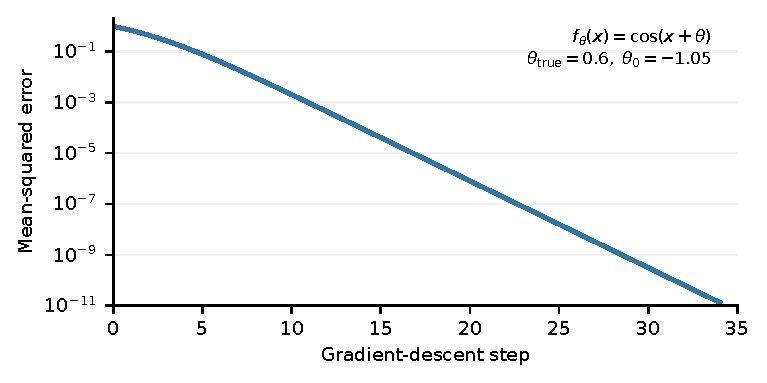
\includegraphics[width=.76\linewidth]{figures/qml/one_qubit_training.pdf}
\caption{Full-batch gradient descent for $f_\theta(x)=\cos(x+\theta)$ using 31 equally spaced inputs in $[-1.35,1.35]$, exact targets $\cos(x+0.6)$, initial $\theta_0=-1.05$, and learning rate $0.34$. The graph plots the exact mean-squared error over 35 steps, without sampling noise.}
\label{fig:qml-training-curve}
\end{figure}
\subsection*{2) Depolarizing noise}
Consider a noise channel on a qubit, after the ideal circuit, that replaces its density operator with a mixture of the original state and the maximally mixed state:
\begin{equation}
 \mathcal E_p(\rho)=(1-p)\rho+p\frac{\mathbf1_2}{2},\qquad0\le p\le1.
\end{equation}
Since $\operatorname{tr}(\sigma_z)=0$, the noisy readout of the previous one-qubit model is
\begin{equation}
 f_{\theta,p}(x)=\operatorname{tr}[\mathcal E_p(\rho_\theta(x))\sigma_z]
 =(1-p)\cos(x+\theta).
\end{equation}
Its parameter derivative is reduced by the same factor $1-p$. Strong depolarization reduces the information about the trainable parameter available through this measurement. The effect is specific to the stated channel and observable; other error processes change predictions in different ways.

\subsection*{3) How many measurements are needed?}
Suppose we want standard error at most $\epsilon$ in a Pauli expectation estimate. The variance inequality in the preceding section implies the sufficient condition
\begin{equation}
 N_{\mathrm{shots}}\ge\epsilon^{-2}.
\end{equation}
For example, $\epsilon=0.01$ requires up to $10^4$ shots for this worst-case variance estimate. To estimate a parameter-shift derivative with two independent batches of $N_{\mathrm{shots}}$ shots, the variance is bounded by $1/(2N_{\mathrm{shots}})$, because each term carries a factor of $1/2$. Training many parameters over many data points may therefore use substantially more circuit executions than one prediction.

\section{Learning from Quantum States}
The use of quantum inputs can be closer to experimental quantum physics than classical-data classification. Suppose an experiment prepares an unknown two-qubit state $\rho$. We would like to determine whether it contains entanglement without reconstructing every matrix entry. One possible test uses an \emph{entanglement witness} associated with the Bell state $\ket{\Phi^+}=(\ket{00}+\ket{11})/\sqrt2$:
\begin{equation}
 \op W=\frac12\mathbf1_4-\ket{\Phi^+}\bra{\Phi^+}.
\end{equation}
For every pure product state $\ket a\otimes\ket b$, the squared overlap with $\ket{\Phi^+}$ is at most $1/2$. Indeed,
\begin{equation}
|\braket{\Phi^+}{a,b}|^2
=\frac12\bigl|a_0b_0+a_1b_1\bigr|^2\le\frac12,
\end{equation}
by the Cauchy--Schwarz inequality and the normalization of each qubit. A separable mixed state is a convex combination of product states, so it also satisfies $\operatorname{tr}(\rho\op W)\ge0$. Therefore
\begin{equation}
 \boxed{\operatorname{tr}(\rho\op W)<0
 \quad\Longrightarrow\quad\rho\text{ is entangled}.}
\end{equation}
This is a useful classification statement about genuinely quantum data: the expectation of a Hermitian operator witnesses a physically meaningful property. Some entangled states will not be detected by this particular witness, since the criterion is sufficient but not necessary.

The operator $\op W$ can be decomposed into Pauli products,
\begin{equation}
\ket{\Phi^+}\bra{\Phi^+}
=\frac14\bigl(\mathbf1\otimes\mathbf1+
\sigma_x\otimes\sigma_x-\sigma_y\otimes\sigma_y+
\sigma_z\otimes\sigma_z\bigr),
\end{equation}
so its expectation can be estimated from local correlation measurements. This directly connects quantum learning tasks with the density-matrix, Bell-state and measurement material introduced earlier in the textbook.

\clearpage
\section{Statistical Concentration and a Trainability Check}
Why do randomly chosen circuits sometimes provide little training information? Let $\ket\psi$ be a Haar-random pure state in a $d$-dimensional Hilbert space, and let $\op O$ be a traceless Hermitian observable. Then the second moment of the random state gives
\begin{equation}
 \mathbb E\bigl[\langle\op O\rangle_\psi\bigr]=0,
 \qquad
 \operatorname{Var}\bigl[\langle\op O\rangle_\psi\bigr]
 =\frac{\operatorname{tr}(\op O^2)}{d(d+1)}.
\end{equation}
For an $n$-qubit Pauli string with eigenvalues $\pm1$, $d=2^n$ and $\operatorname{tr}(\op O^2)=d$, so
\begin{equation}
 \boxed{\operatorname{Var}\bigl[\langle\op O\rangle_\psi\bigr]
 =\frac1{2^n+1}.}
\end{equation}
Thus expectation values of a fixed traceless observable concentrate near zero under uniformly random pure states in high dimension. We can also examine a particular derivative rather than the expectation of a Pauli observable. Draw $\ket\psi$ from the Haar distribution in dimension $d=2^n$, apply $e^{-\ii\theta X_1/2}$, and measure the probability $f(\theta)=|\bra{0^n}e^{-\ii\theta X_1/2}\ket\psi|^2$. Here $X_1$ acts on the first qubit. If $a=\langle 0^n|\psi\rangle$ and $b=\langle 10^{n-1}|\psi\rangle$, then $f'(0)=\operatorname{Im}(a^*b)$. The Haar fourth moment yields
\begin{equation}
\boxed{\operatorname{Var}[f'(0)]=\frac{1}{2d(d+1)},\qquad d=2^n.}
\end{equation}
\begin{figure}[htbp]
\centering
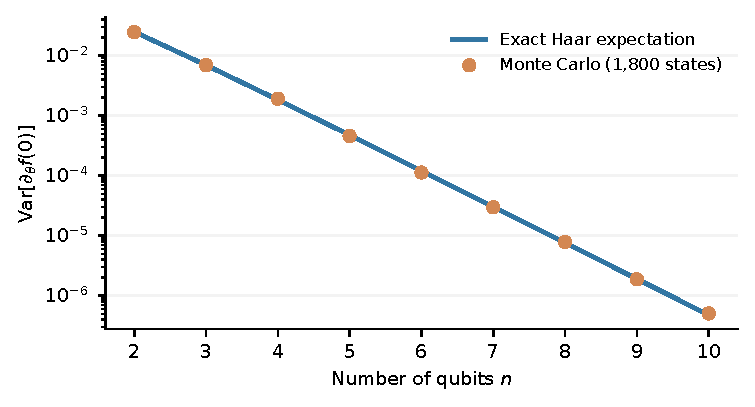
\includegraphics[width=.75\linewidth]{figures/qml/global_projector_gradients.pdf}
\caption{Gradient concentration for this specific global-projector objective: exact Haar variance $[2d(d+1)]^{-1}$ versus 1,800 independent numerically sampled Haar states at each $n$. This illustrative ensemble of random states is a precisely defined toy model, not a universal statement about practical QNN architectures.}
\label{fig:qml-global-gradient}
\end{figure}

This calculation by itself is \emph{not} a barren-plateau theorem for derivatives, but it illustrates the concentration mechanism underlying many rigorous gradient-suppression results~\cite{McClean2018,Larocca2025}. The correct gradient scaling depends on the circuit generators, initial state, measurement locality, and objective function.